\documentclass[12pt,a4paper]{article}

% -- Packages ------------------------------------------------------
\usepackage[T1]{fontenc}
\usepackage[utf8]{inputenc}
\usepackage[english]{babel}
\usepackage{geometry}
\geometry{margin=2.5cm, top=3cm, bottom=3cm}

\usepackage{amsmath, amssymb}
\usepackage{graphicx}
\usepackage{xcolor}
\usepackage{listings}
\usepackage{tcolorbox}
\tcbuselibrary{listings, skins, breakable}
\usepackage{hyperref}
\usepackage{booktabs}
\usepackage{array}
\usepackage{enumitem}
\usepackage{fancyhdr}
\usepackage{titlesec}
\usepackage{mdframed}
\usepackage{tikz}
\usetikzlibrary{shapes.geometric, arrows.meta, fit, positioning, backgrounds}

% -- Colors --------------------------------------------------------
\definecolor{primary}{RGB}{31, 78, 121}
\definecolor{accent}{RGB}{0, 147, 221}
\definecolor{codegreen}{RGB}{40, 167, 69}
\definecolor{codegray}{RGB}{108, 117, 125}
\definecolor{codepurple}{RGB}{111, 66, 193}
\definecolor{codebg}{RGB}{248, 249, 250}
\definecolor{warningbg}{RGB}{255, 248, 220}
\definecolor{warningborder}{RGB}{255, 193, 7}
\definecolor{infobg}{RGB}{219, 234, 254}
\definecolor{infoborder}{RGB}{59, 130, 246}
\definecolor{successbg}{RGB}{209, 250, 229}
\definecolor{successborder}{RGB}{16, 185, 129}
\definecolor{notebookbg}{RGB}{240, 247, 255}

% -- Page Style ----------------------------------------------------
\pagestyle{fancy}
\fancyhf{}
\fancyhead[L]{\small\color{primary}\textbf{Machine Fault Recognition --- Notebook Guide}}
\fancyhead[R]{\small\color{codegray}\thepage}
\fancyfoot[C]{\small\color{codegray}\hrule\vspace{2pt} Complete Guide to DBSCAN Clustering \& EfficientNet Classification}
\renewcommand{\headrulewidth}{0.4pt}

% -- Section Formatting --------------------------------------------
\titleformat{\section}{\Large\bfseries\color{primary}}{}{0em}{\thesection\quad}[\titlerule]
\titleformat{\subsection}{\large\bfseries\color{accent}}{}{0em}{\thesubsection\quad}
\titleformat{\subsubsection}{\normalsize\bfseries\color{primary}}{}{0em}{\thesubsubsection\quad}

% -- Code Listing Style --------------------------------------------
\lstdefinestyle{pythonstyle}{
  language=Python,
  backgroundcolor=\color{codebg},
  commentstyle=\color{codegreen}\itshape,
  keywordstyle=\color{codepurple}\bfseries,
  stringstyle=\color{accent},
  numberstyle=\tiny\color{codegray},
  basicstyle=\ttfamily\small,
  breakatwhitespace=false,
  breaklines=true,
  captionpos=b,
  keepspaces=true,
  numbers=left,
  numbersep=8pt,
  showspaces=false,
  showstringspaces=false,
  showtabs=false,
  tabsize=4,
  frame=single,
  rulecolor=\color{accent!40},
  xleftmargin=15pt,
  framexleftmargin=10pt,
  morekeywords={import, from, as, def, class, return, if, else, elif, for, in, with, True, False, None, not, and, or, self, super, print, len, range, int, float, str, list, dict, set, tuple, type, isinstance, assert, raise, try, except, finally, lambda, yield}
}
\lstset{style=pythonstyle}

% -- Custom Box Environments ---------------------------------------
\newmdenv[
  backgroundcolor=infobg,
  linecolor=infoborder,
  linewidth=2pt,
  leftline=true, rightline=false, topline=false, bottomline=false,
  innerleftmargin=10pt, innerrightmargin=10pt,
  innertopmargin=8pt, innerbottommargin=8pt,
]{infobox}

\newmdenv[
  backgroundcolor=warningbg,
  linecolor=warningborder,
  linewidth=2pt,
  leftline=true, rightline=false, topline=false, bottomline=false,
  innerleftmargin=10pt, innerrightmargin=10pt,
  innertopmargin=8pt, innerbottommargin=8pt,
]{warningbox}

\newmdenv[
  backgroundcolor=successbg,
  linecolor=successborder,
  linewidth=2pt,
  leftline=true, rightline=false, topline=false, bottomline=false,
  innerleftmargin=10pt, innerrightmargin=10pt,
  innertopmargin=8pt, innerbottommargin=8pt,
]{successbox}

\newmdenv[
  backgroundcolor=notebookbg,
  linecolor=primary,
  linewidth=1pt,
  roundcorner=4pt,
  innerleftmargin=12pt, innerrightmargin=12pt,
  innertopmargin=10pt, innerbottommargin=10pt,
]{notebookbox}

% -- Hyperref Setup ------------------------------------------------
\hypersetup{
  colorlinks=true,
  linkcolor=primary,
  urlcolor=accent,
  citecolor=codegreen,
  pdftitle={Machine Fault Recognition --- Complete Notebook Guide},
  pdfauthor={},
}

% -----------------------------------------------------------------
\begin{document}
% -----------------------------------------------------------------

%% ================================================================
%%  TITLE PAGE
%% ================================================================
\begin{titlepage}
  \centering
  \vspace*{1.5cm}
  {\Huge\bfseries\color{primary} Machine Fault Recognition\par}
  \vspace{0.5cm}
  {\LARGE\color{accent} Complete Notebook Guide\par}
  \vspace{0.3cm}
  \textcolor{codegray}{\rule{0.6\textwidth}{1.5pt}}
  \vspace{0.8cm}

  \begin{tcolorbox}[
    colback=notebookbg, colframe=primary, arc=6pt,
    width=0.85\textwidth, boxrule=1pt
  ]
  \centering
  \textbf{\large Notebook 1:} \textit{DBSCAN Acoustic Clustering} \\[4pt]
  \footnotesize Unsupervised grouping of machine recordings using hand-crafted acoustic features,
  dimensionality reduction (PCA + UMAP), and DBSCAN to detect physical recording events.
  \vspace{8pt}

  \textbf{\large Notebook 2:} \textit{EfficientNet Cluster-Aware Split} \\[4pt]
  \footnotesize Deep learning classifier (EfficientNet-B0 + Temporal Attention) trained with
  a strict grouped split that prevents data leakage across cluster boundaries.
  \end{tcolorbox}

  \vspace{1cm}
  \begin{successbox}
    \textbf{What you will learn:}
    \begin{itemize}[leftmargin=*, nosep]
      \item How DBSCAN discovers natural recording events in acoustic data
      \item Why naive train/test splits cause inflated accuracy (data leakage)
      \item How to build a deep audio classifier with PyTorch and EfficientNet
      \item How to write, understand, and reproduce both notebooks yourself
    \end{itemize}
  \end{successbox}

  \vfill
  {\color{codegray}\today}
\end{titlepage}

\tableofcontents
\newpage

%% ================================================================
\section{Project Overview and Motivation}
%% ================================================================

\subsection{The Problem Being Solved}

Consider a factory with three rotating machines, each of which can operate in a \textbf{normal} or \textbf{abnormal} (faulty) state. The task is to build a classifier that listens to short audio clips of these machines and determines which machine is operating and whether it is healthy.

The dataset has \textbf{6 classes}: M1-Normal, M1-Abnormal, M2-Normal, M2-Abnormal, M3-Normal, M3-Abnormal.

The challenge lies not in the classifier design alone, but in \textbf{how the data is split}. Audio datasets recorded in the wild often contain many segments from the same physical recording session. If a 10-minute recording is cut into 344 one-second segments, those segments are highly correlated. Randomly splitting them into train/test means the model essentially memorizes the recording rather than learning to generalize --- this is called \textbf{data leakage}.

\begin{warningbox}
\textbf{The Data Leakage Problem:} Randomly shuffling and splitting audio segments can produce test accuracy close to 100\% even though the model has learned nothing. Segments from the same recording appear in both train and test sets, so the model just recognizes the recording session, not the machine fault.
\end{warningbox}

\subsection{The Two-Notebook Solution}

The solution is elegant and consists of two stages run in order:

\begin{center}
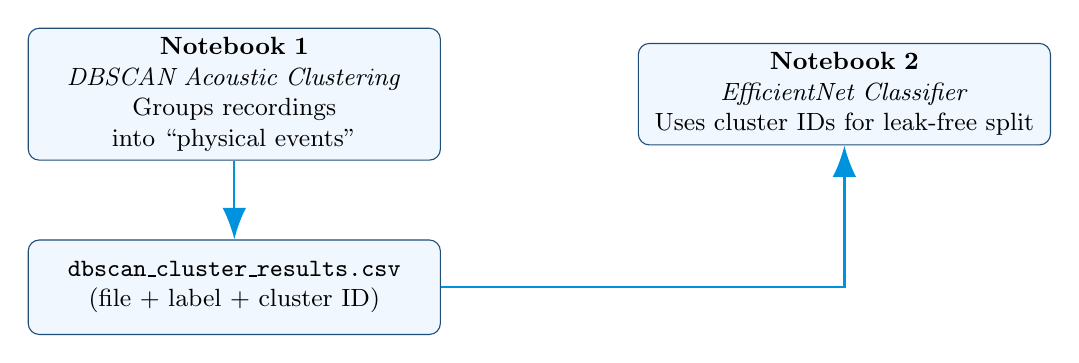
\begin{tikzpicture}[
  node distance=1.2cm,
  box/.style={rectangle, rounded corners=4pt, draw=primary, fill=notebookbg,
              text width=5cm, align=center, minimum height=1.2cm, font=\small},
  arrow/.style={-{Latex[length=4mm]}, thick, color=accent}
]
\node[box] (nb1) {\textbf{Notebook 1}\\\textit{DBSCAN Acoustic Clustering}\\Groups recordings into ``physical events''};
\node[box, right=2.5cm of nb1] (nb2) {\textbf{Notebook 2}\\\textit{EfficientNet Classifier}\\Uses cluster IDs for leak-free split};
\node[box, below=1.0cm of nb1] (csv) {\texttt{dbscan\_cluster\_results.csv}\\(file + label + cluster ID)};
\draw[arrow] (nb1) -- (csv);
\draw[arrow] (csv) -| (nb2);
\end{tikzpicture}
\end{center}

\vspace{6pt}
\begin{enumerate}
  \item \textbf{Notebook 1} analyses the acoustic properties of every \texttt{.wav} file, reduces the dimensionality of the resulting feature vectors, and runs DBSCAN to label each file with a \textit{cluster ID} that represents its physical recording session.
  \item \textbf{Notebook 2} loads the CSV produced by Notebook 1, uses the cluster IDs to split the data so that no cluster appears in more than one split, and then trains a deep neural network classifier.
\end{enumerate}


%% ================================================================
\section{Notebook 1 --- DBSCAN Acoustic Clustering}
%% ================================================================

\begin{notebookbox}
\textbf{File:} \texttt{dbscan\_acoustic\_clustering.ipynb} \quad
\textbf{Runtime:} CPU only (no GPU needed) \quad
\textbf{Output:} \texttt{dbscan\_cluster\_results.csv}, several PNG plots
\end{notebookbox}

\subsection{What This Notebook Does --- Big Picture}

The notebook answers one question: \textit{``Which audio files were recorded in the same physical recording session?''}

It does this without any labels, using only the acoustic content of the files. The pipeline is:

\[
\text{Raw .wav} \xrightarrow{\text{librosa}} \text{232-dim feature vector} \xrightarrow{\text{StandardScaler}} \text{scaled} \xrightarrow{\text{PCA}} \text{reduced} \xrightarrow{\text{UMAP}} \text{15-D} \xrightarrow{\text{DBSCAN}} \text{cluster ID}
\]

\subsection{Section 1 --- Imports and Configuration}

\subsubsection{Libraries Used}

\begin{center}
\begin{tabular}{ll}
\toprule
\textbf{Library} & \textbf{Role} \\
\midrule
\texttt{librosa} & Audio loading and acoustic feature extraction \\
\texttt{sklearn} & StandardScaler, PCA, DBSCAN, NearestNeighbors, metrics \\
\texttt{umap-learn} & Non-linear dimensionality reduction \\
\texttt{numpy} & Numerical arrays \\
\texttt{pandas} & Tabular data (the results CSV) \\
\texttt{matplotlib / seaborn} & Visualizations \\
\texttt{concurrent.futures} & Parallel feature extraction across CPU cores \\
\bottomrule
\end{tabular}
\end{center}

\subsubsection{Key Constants You Should Understand}

\begin{lstlisting}
TARGET_SR      = 16000       # Resample all audio to 16 kHz
TARGET_SAMPLES = TARGET_SR * 11  # Pad/trim every clip to exactly 11 s
N_MFCC         = 40          # Number of MFCC coefficients
N_MELS         = 64          # Mel bands for the spectrogram stats
N_FFT          = 1024        # FFT window size (~64 ms at 16 kHz)
HOP_LENGTH     = 512         # Hop (overlap) between frames
N_CHROMA       = 12          # Chroma bins (one per semitone)
MAX_WORKERS    = 4           # Parallel CPU workers for extraction
\end{lstlisting}

\begin{infobox}
\textbf{Why 16 kHz?} The human voice and many machine sounds have most energy below 8 kHz. By resampling to 16 kHz (Nyquist: 8 kHz) we discard inaudible high-frequency content and reduce computation. \\[4pt]
\textbf{Why 11 seconds?} The dataset recordings are approximately 11 s long. Fixing a length allows stacking all feature vectors into a single numpy matrix.
\end{infobox}

\subsubsection{How to Write This Section Yourself}

\begin{enumerate}
  \item Import the libraries at the top of the notebook.
  \item Detect whether you are on Kaggle (\texttt{os.path.exists('/kaggle/input')}) to set paths dynamically.
  \item Define all hyperparameters as uppercase global constants --- this makes them easy to find and change.
\end{enumerate}

\subsection{Section 2 --- Discovering Audio Files and Inferring Labels}

\begin{lstlisting}
# Discover all .wav files recursively under SAMP_DIR
wav_files = sorted([str(p) for p in Path(SAMP_DIR).rglob('*.wav')])
\end{lstlisting}

The \texttt{infer\_label} function parses the folder path to extract the machine number and state:

\begin{lstlisting}
def infer_label(filepath: str):
    parts = filepath.lower().replace('\\', '/').split('/')
    machine_num = 0
    for p in parts:
        if 'machine_1' in p or 'machine 1' in p: machine_num = 1; break
        if 'machine_2' in p or 'machine 2' in p: machine_num = 2; break
        if 'machine_3' in p or 'machine 3' in p: machine_num = 3; break
    state = 'abnormal' if any('abnormal' in p for p in parts) else 'normal'
    base  = (machine_num - 1) * 2 if machine_num > 0 else 0
    label = base + (1 if state == 'abnormal' else 0)
    return label, machine_num, state
\end{lstlisting}

\begin{infobox}
\textbf{Label encoding:} M1-Normal=0, M1-Abnormal=1, M2-Normal=2, M2-Abnormal=3, M3-Normal=4, M3-Abnormal=5. The formula \texttt{base + (1 if abnormal else 0)} with \texttt{base=(machine-1)*2} generates this automatically.
\end{infobox}

\subsection{Section 3 --- Acoustic Feature Extraction (232 Dimensions)}

This is the most important section of Notebook 1. For each \texttt{.wav} file the function \texttt{extract\_features} computes a 232-dimensional vector capturing different aspects of the sound.

\subsubsection{Understanding Each Feature Group}

\paragraph{1. MFCCs --- 120 dimensions}
Mel-Frequency Cepstral Coefficients capture the \textit{timbre} (tone quality) of the sound. The 40 coefficients represent the spectral envelope of the audio.

\begin{lstlisting}
mfcc       = librosa.feature.mfcc(y=y, sr=sr, n_mfcc=N_MFCC, ...)
mfcc_delta = librosa.feature.delta(mfcc)      # rate of change
feats.extend(mfcc.mean(axis=1))               # 40 values: average per coeff
feats.extend(mfcc.std(axis=1))                # 40 values: variability
feats.extend(mfcc_delta.mean(axis=1))         # 40 values: average change rate
\end{lstlisting}

\paragraph{2. Spectral Features --- 8 dimensions}
These describe the \textit{shape} of the frequency spectrum:

\begin{center}
\begin{tabular}{ll}
\toprule
\textbf{Feature} & \textbf{What it measures} \\
\midrule
Spectral Centroid & Average frequency (brightness) \\
Spectral Bandwidth & Spread of frequencies around centroid \\
Spectral Rolloff & Frequency below which 85\% of energy lies \\
Spectral Flatness & How noise-like vs. tonal the sound is \\
\bottomrule
\end{tabular}
\end{center}

Each feature contributes mean + std = 2 values, total = 8.

\paragraph{3. Zero-Crossing Rate --- 2 dimensions}
How often the waveform crosses zero. High ZCR indicates noisy or percussive sound.

\paragraph{4. RMS Energy --- 2 dimensions}
Root Mean Square amplitude. Measures overall loudness.

\paragraph{5. Chroma Features --- 24 dimensions}
Represent the energy in each of the 12 musical pitch classes (C, C\#, D, ..., B). Mean + std per bin = 24.

\paragraph{6. Mel-Spectrogram Statistics --- 64 dimensions}
Mean and standard deviation of each of 32 Mel frequency bands in the power spectrogram.

\paragraph{7. Tonnetz --- 12 dimensions}
Harmonic network representation capturing tonal relationships (sixths, thirds, perfect fifths).

\subsubsection{Parallel Extraction}

\begin{lstlisting}
with ProcessPoolExecutor(max_workers=MAX_WORKERS) as ex:
    futures = {ex.submit(extract_features, fp): i for i, fp in enumerate(file_list)}
    for fut in tqdm(as_completed(futures), total=len(futures)):
        i = futures[fut]
        results[i] = fut.result()   # None if the file failed to load
\end{lstlisting}

The results are also cached to a \texttt{.npz} file so re-running the notebook skips extraction.

\subsection{Section 4 --- Cleaning Features}

\begin{lstlisting}
# Replace NaN/Inf values with the column median
for col in range(X_clean.shape[1]):
    bad = ~np.isfinite(X_clean[:, col])
    if bad.any():
        X_clean[bad, col] = np.nanmedian(X_clean[:, col])

# Remove features that are constant (zero variance) --- they carry no information
var       = X_clean.var(axis=0)
keep_mask = var > 1e-8
X_clean   = X_clean[:, keep_mask]
\end{lstlisting}

\subsection{Section 5 --- Dimensionality Reduction}

232 dimensions is too many for DBSCAN to work well (the \textit{curse of dimensionality}: distances become meaningless in high dimensions). The notebook reduces dimensions in two steps.

\subsubsection{Step 1: StandardScaler}
Normalises each feature to zero mean and unit variance. Without this, features with large numerical ranges (e.g., RMS energy in dB) dominate the distance calculations.

\begin{lstlisting}
scaler   = StandardScaler()
X_scaled = scaler.fit_transform(X_clean)
\end{lstlisting}

\subsubsection{Step 2: PCA}
Principal Component Analysis projects data onto orthogonal axes that explain the most variance. \texttt{n\_components=0.95} keeps enough components to retain 95\% of the variance.

\begin{lstlisting}
pca   = PCA(n_components=0.95, random_state=SEED)
X_pca = pca.fit_transform(X_scaled)
# Typically reduces ~232 dims to ~30-60 principal components
\end{lstlisting}

\subsubsection{Step 3: UMAP}
UMAP (Uniform Manifold Approximation and Projection) is a non-linear dimensionality reduction method that preserves local neighbourhood structure. Two UMAP embeddings are computed:

\begin{lstlisting}
# 15D for DBSCAN --- enough structure, low enough for good distance metrics
reducer_nd = umap.UMAP(n_components=15, n_neighbors=30,
                        min_dist=0.0, metric='euclidean', ...)
X_umap_nd  = reducer_nd.fit_transform(X_pca)

# 2D for plotting only
reducer_2d = umap.UMAP(n_components=2, n_neighbors=30, min_dist=0.1, ...)
X_umap_2d  = reducer_2d.fit_transform(X_pca)
\end{lstlisting}

\begin{infobox}
\textbf{Key UMAP parameters:}
\begin{itemize}[nosep]
  \item \texttt{n\_neighbors}: controls the local/global balance. Higher = more global structure.
  \item \texttt{min\_dist}: minimum distance in embedded space. \texttt{0.0} = tighter clusters (good for DBSCAN). \texttt{0.1} = more spread (good for visualization).
\end{itemize}
\end{infobox}

\subsection{Section 6 --- DBSCAN Parameter Tuning (k-NN Distance Plot)}

DBSCAN requires two parameters: \texttt{eps} (neighbourhood radius) and \texttt{min\_samples} (minimum points in a neighbourhood). The k-NN distance plot helps choose \texttt{eps}:

\begin{lstlisting}
K = max(5, X_umap_nd.shape[1] * 2)   # rule of thumb: minPts >= 2 * dims
nbrs    = NearestNeighbors(n_neighbors=K).fit(X_umap_nd)
dists,_ = nbrs.kneighbors(X_umap_nd)
k_dists = np.sort(dists[:, K-1])[::-1]   # K-th nearest neighbour distance
\end{lstlisting}

The sorted distances are plotted; the \textit{elbow} (point of maximum curvature) suggests the optimal \texttt{eps}: points to the left are dense (core points), points to the right are sparse (noise).

\subsection{Section 7 --- Grid Search over eps x min\_samples}

\begin{lstlisting}
for eps in eps_candidates:
    for ms in min_samples_range:
        labels = DBSCAN(eps=eps, min_samples=ms).fit_predict(X_umap_nd)
        n_cl   = len(set(labels)) - (1 if -1 in labels else 0)
        # Compute silhouette, Davies-Bouldin, ARI, NMI
\end{lstlisting}

\subsubsection{Evaluation Metrics}

\begin{center}
\begin{tabular}{lll}
\toprule
\textbf{Metric} & \textbf{Range} & \textbf{What ``good'' looks like} \\
\midrule
Silhouette Score & $[-1, +1]$ & High (close to +1) \\
Davies-Bouldin Index & $[0, \infty)$ & Low (close to 0) \\
Adjusted Rand Index (ARI) & $[-1, +1]$ & High (agrees with true labels) \\
Norm. Mutual Information & $[0, 1]$ & High (shares information with labels) \\
\bottomrule
\end{tabular}
\end{center}

\subsection{Section 8 --- Final DBSCAN Run}

The best parameter combination is selected automatically by combining silhouette score and noise fraction:

\begin{lstlisting}
# Auto-select: good silhouette, < 25% noise, >= 2 clusters
valid_rows = res_df[(res_df['n_clusters'] >= 2) & (res_df['noise_%'] < 25)]
best_row   = valid_rows.iloc[0]  # sorted by score descending

db_final      = DBSCAN(eps=BEST_EPS, min_samples=BEST_MS)
cluster_labels = db_final.fit_predict(X_umap_nd)
df['cluster']  = cluster_labels   # -1 = noise
\end{lstlisting}

\begin{warningbox}
\textbf{Noise points (cluster = -1):} DBSCAN labels points that do not belong to any dense region as noise. These are \textit{dropped} in Notebook 2 before the grouped split. Do not worry if 5--20\% of files are noise --- this is expected and healthy.
\end{warningbox}

\subsection{Sections 9--11 --- Visualisations and Output}

The notebook produces six plots:
\begin{enumerate}[nosep]
  \item 2x2 UMAP overview (clusters, ground truth, machine, normal/abnormal)
  \item Cluster $\times$ true-label heatmap
  \item Per-cluster machine + state stacked bar charts
  \item Cluster sizes with dominant class annotation
  \item UMAP faceted by machine
  \item Grid-search heatmap (silhouette, n\_clusters, noise\%)
\end{enumerate}

The final output is \texttt{dbscan\_cluster\_results.csv} with columns:
\texttt{file\_path | label | machine | state | class\_name | cluster | umap\_x | umap\_y}


%% ================================================================
\section{Notebook 2 --- EfficientNet with Cluster-Aware Split}
%% ================================================================

\begin{notebookbox}
\textbf{File:} \texttt{EfficientNet\_clustered\_split.ipynb} \quad
\textbf{Runtime:} GPU recommended (CUDA) \quad
\textbf{Input:} \texttt{dbscan\_cluster\_results.csv} from Notebook 1
\end{notebookbox}

\subsection{What This Notebook Does --- Big Picture}

Notebook 2 trains a deep learning model to classify machine faults. Its defining feature is the \textbf{cluster-aware split}: instead of randomly shuffling audio segments, it groups them by DBSCAN cluster ID and ensures every cluster goes entirely into one split (train, val, or test).

The model architecture is called \textbf{EfficientNet}:

\begin{center}
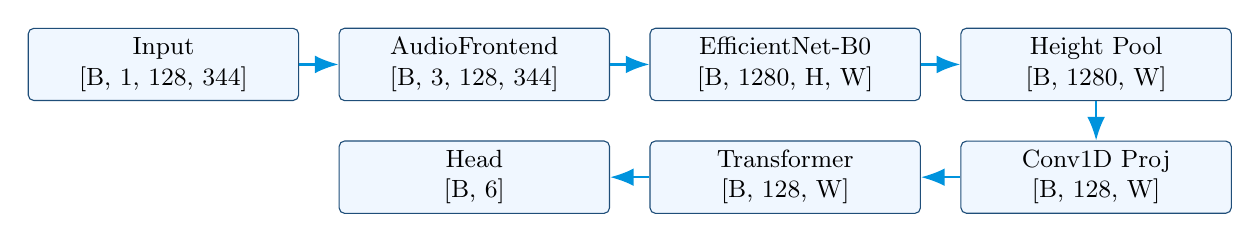
\begin{tikzpicture}[
  node distance=0.4cm and 0.2cm,
  block/.style={rectangle, rounded corners=2pt, draw=primary, fill=notebookbg,
                text width=3.2cm, align=center, font=\small, minimum height=0.9cm},
  arr/.style={-{Latex[length=3mm]}, thick, color=accent}
]
\node[block] (in) {Input\\{[B, 1, 128, 344]}};
\node[block, right=0.5cm of in] (fe) {AudioFrontend\\{[B, 3, 128, 344]}};
\node[block, right=0.5cm of fe] (eff) {EfficientNet-B0\\{[B, 1280, H, W]}};
\node[block, right=0.5cm of eff] (pool) {Height Pool\\{[B, 1280, W]}};
\node[block, below=0.5cm of pool] (proj) {Conv1D Proj\\{[B, 128, W]}};
\node[block, left=0.5cm of proj] (attn) {Transformer\\{[B, 128, W]}};
\node[block, left=0.5cm of attn] (head) {Head\\{[B, 6]}};

\draw[arr] (in) -- (fe);
\draw[arr] (fe) -- (eff);
\draw[arr] (eff) -- (pool);
\draw[arr] (pool) -- (proj);
\draw[arr] (proj) -- (attn);
\draw[arr] (attn) -- (head);
\end{tikzpicture}
\end{center}

\subsection{Section 1 --- Imports and Configuration}

\subsubsection{Key Configuration Constants}

\begin{lstlisting}
CLUSTER_CSV_PATH = '/kaggle/input/your-dataset/dbscan_cluster_results.csv'
USE_PRECOMPUTED_NPY = False   # True = load .npy Mel spectrograms (fast)

SAMPLE_RATE   = 16_000        # Must match Notebook 1
DURATION_SEC  = 11.0
N_MELS        = 128           # More Mel bands than NB1 (richer features)
N_FFT         = 1024
HOP_LENGTH    = 512
TARGET_FRAMES = 344           # ceil(16000 * 11 / 512)

BATCH_SIZE  = 32
EPOCHS      = 40
LR          = 1e-3
NUM_CLASSES = 6
\end{lstlisting}

\begin{infobox}
\textbf{Two input modes:}
\begin{itemize}[nosep]
  \item \texttt{USE\_PRECOMPUTED\_NPY=False}: The Dataset class loads raw \texttt{.wav} files and computes Mel spectrograms on the fly using librosa. Slower but requires no pre-processing step.
  \item \texttt{USE\_PRECOMPUTED\_NPY=True}: Loads pre-saved \texttt{.npy} arrays. Much faster on Kaggle T4 GPUs.
\end{itemize}
\end{infobox}

\subsection{Section 2 --- Data Loading and Strict Grouped Split}

This is the most critical section of Notebook 2. The key insight is to use \texttt{GroupShuffleSplit} with cluster IDs as groups.

\subsubsection{Step-by-Step}

\begin{lstlisting}
df_all   = pd.read_csv(CLUSTER_CSV_PATH)
df_clean = df_all[df_all['cluster'] != -1]   # drop DBSCAN noise points

# Encode string labels -> integers
label_map        = {name: idx for idx, name in enumerate(CLASS_NAMES)}
df_clean['label_int'] = df_clean['label'].map(label_map)

groups = df_clean['cluster'].values   # <-- the crucial grouping key

# Pass 1: 70% train vs 30% temp (val+test)
gss1 = GroupShuffleSplit(n_splits=1, train_size=0.70, random_state=SEED)
train_idx, temp_idx = next(gss1.split(df_clean, groups=groups))

# Pass 2: split the 30% temp into 15% val and 15% test
gss2 = GroupShuffleSplit(n_splits=1, train_size=0.50, random_state=SEED)
val_idx, test_idx = next(gss2.split(df_temp, groups=df_temp['cluster'].values))
\end{lstlisting}

\subsubsection{Leak Verification}

\begin{lstlisting}
# Guarantee zero overlap --- this assertion would crash if leakage existed
assert train_c.isdisjoint(val_c),  'Train/Val cluster overlap!'
assert train_c.isdisjoint(test_c), 'Train/Test cluster overlap!'
assert val_c.isdisjoint(test_c),   'Val/Test cluster overlap!'
\end{lstlisting}

\begin{successbox}
\textbf{Why this matters:} With 94 physical clusters split 70/15/15, the test set contains entirely different recording sessions from training. Accuracy on this test set reflects genuine generalisation, not memorized recording artifacts.
\end{successbox}

\subsection{Section 3 --- The MachineAudioDataset Class}

The \texttt{Dataset} class bridges the CSV metadata to the PyTorch DataLoader.

\begin{lstlisting}
class MachineAudioDataset(Dataset):
    def __getitem__(self, idx):
        row  = self.df.iloc[idx]
        path = row['file_path']

        # Load either .wav (slow) or .npy (fast)
        if self.use_npy:
            mel_np = np.load(path).astype(np.float32)
        else:
            y, sr = librosa.load(path, sr=SAMPLE_RATE, duration=DURATION_SEC)
            mel_np = librosa.feature.melspectrogram(y=y, sr=sr, ...)
            mel_np = librosa.power_to_db(mel_np, ref=np.max)

        mel_np = self._fix_time(mel_np)   # ensure [128, 344]

        # Normalise to [-1, 1] per sample
        lo, hi = mel_np.min(), mel_np.max()
        if hi > lo:
            mel_np = 2.0 * (mel_np - lo) / (hi - lo) - 1.0

        mel = torch.from_numpy(mel_np).unsqueeze(0)  # [1, 128, 344]

        # SpecAugment during training only
        if self.augment:
            mel = self.time_mask(self.freq_mask(mel))

        return mel, int(row['label_int'])
\end{lstlisting}

\subsubsection{SpecAugment}
SpecAugment is a simple but powerful data augmentation for audio. It randomly masks rectangular bands in time and frequency:

\begin{center}
\begin{tabular}{ll}
\toprule
\textbf{Augmentation} & \textbf{Effect} \\
\midrule
\texttt{FrequencyMasking(freq\_mask\_param=15)} & Zeros up to 15 frequency bins \\
\texttt{TimeMasking(time\_mask\_param=35)} & Zeros up to 35 time frames \\
\bottomrule
\end{tabular}
\end{center}

\subsection{Section 4 --- DataLoaders with Class-Balanced Sampling}

\begin{lstlisting}
# Compute inverse-frequency weights
counts        = df_train.groupby('label_int').size()
class_weights = torch.tensor([1.0 / counts[i] for i in range(NUM_CLASSES)])
sample_weights = [float(class_weights[int(l)]) for l in df_train['label_int']]

# WeightedRandomSampler: rare classes sampled more often
sampler = WeightedRandomSampler(sample_weights,
                                num_samples=len(sample_weights),
                                replacement=True)
\end{lstlisting}

\begin{infobox}
\textbf{Why class balancing?} If abnormal sounds are rarer than normal sounds, a naive model might just predict ``normal'' for everything and still achieve high accuracy. Oversampling minority classes forces the model to learn all 6 classes equally.
\end{infobox}

\subsection{Section 5 --- EfficientNet Model Architecture}

The model has four main components:

\subsubsection{Component 1: AudioFrontend}

Converts a single-channel Mel spectrogram into three channels by appending delta and delta-delta features:

\begin{lstlisting}
class AudioFrontend(nn.Module):
    def forward(self, x):               # x: [B, 1, F, T]
        delta  = torchaudio.functional.compute_deltas(x)
        delta2 = torchaudio.functional.compute_deltas(delta)
        return torch.cat([x, delta, delta2], dim=1)  # [B, 3, F, T]
\end{lstlisting}

\begin{infobox}
\textbf{Deltas:} The delta (first derivative) captures how fast the spectrogram is changing. The delta-delta (second derivative) captures acceleration. Together with the original, this gives the model temporal context --- like looking at position, velocity, and acceleration of a moving object.
\end{infobox}

\subsubsection{Component 2: EfficientNet-B0 Backbone}

EfficientNet-B0 is a lightweight image classification CNN loaded from \texttt{timm} (PyTorch Image Models). The \textit{top classifier} is removed (\texttt{num\_classes=0}) and \textit{global pooling} is disabled (\texttt{global\_pool=''}) so we get the spatial feature map.

\begin{lstlisting}
self.backbone = timm.create_model(
    'efficientnet_b0',
    pretrained=False,    # train from scratch
    in_chans=3,          # matches AudioFrontend output
    num_classes=0,       # remove classifier head
    global_pool=''       # keep [B, 1280, H, W] feature map
)
\end{lstlisting}

\subsubsection{Component 3: Temporal Attention (Transformer)}

\begin{lstlisting}
# Collapse frequency dim: [B, 1280, H, W] -> [B, 1280, W]
self.height_pool = nn.AdaptiveAvgPool2d((1, None))

# Project channels: 1280 -> 128
self.proj = nn.Sequential(
    nn.Conv1d(1280, d_model, kernel_size=1, bias=False),
    nn.BatchNorm1d(d_model), nn.GELU()
)

# 2-layer Transformer encoder over time axis
enc_layer = nn.TransformerEncoderLayer(
    d_model=128, nhead=4, dim_feedforward=512,
    dropout=0.4, batch_first=True, norm_first=True  # Pre-LN
)
self.attention = nn.TransformerEncoder(enc_layer, num_layers=2)
\end{lstlisting}

The Transformer learns which time frames are most informative for classification --- for example, a fault might only manifest in certain moments of the recording.

\subsubsection{Component 4: Classification Head}

\begin{lstlisting}
self.head = nn.Sequential(
    nn.AdaptiveAvgPool1d(1),   # pool over time -> [B, 128]
    nn.Flatten(),
    nn.Dropout(0.4),           # regularisation
    nn.Linear(128, 6)          # 6 output classes
)
\end{lstlisting}

\subsection{Section 6 --- Training and Validation Loop}

\begin{lstlisting}
def train_one_epoch(model, loader, criterion, optimizer, scheduler):
    model.train()
    for inputs, labels in loader:
        inputs, labels = inputs.to(DEVICE), labels.to(DEVICE)
        optimizer.zero_grad()
        outputs = model(inputs)
        loss    = criterion(outputs, labels)
        loss.backward()
        nn.utils.clip_grad_norm_(model.parameters(), max_norm=1.0)  # safety
        optimizer.step()
        scheduler.step()   # OneCycleLR updates each batch, not each epoch
\end{lstlisting}

\begin{infobox}
\textbf{Gradient clipping} (\texttt{clip\_grad\_norm\_}): Prevents exploding gradients in the Transformer layers. When gradients become very large, they are rescaled to have a maximum norm of 1.0.
\end{infobox}

\subsection{Section 7 --- Loss, Optimizer, and Scheduler}

\begin{lstlisting}
# Label smoothing: prevents overconfident predictions by mixing true label
# with 0.1 probability distributed over all classes
criterion = nn.CrossEntropyLoss(label_smoothing=0.1)

# AdamW: Adam with decoupled weight decay (better regularisation)
optimizer = optim.AdamW(model.parameters(), lr=1e-3, weight_decay=1e-2)

# OneCycleLR: linearly warms up LR for 30% of training, then anneals
scheduler = optim.lr_scheduler.OneCycleLR(
    optimizer, max_lr=LR,
    steps_per_epoch=len(train_loader), epochs=EPOCHS, pct_start=0.3
)
\end{lstlisting}

\subsubsection{Early Stopping}

\begin{lstlisting}
class EarlyStopping:
    def __init__(self, patience=8, min_delta=0.001):
        self.patience  = patience    # stop after 8 non-improving epochs
        self.min_delta = min_delta   # must improve by at least 0.001
        self.counter   = 0
        self.best_loss = float('inf')

    def __call__(self, val_loss):
        if val_loss < self.best_loss - self.min_delta:
            self.best_loss = val_loss
            self.counter   = 0
        else:
            self.counter += 1
            if self.counter >= self.patience:
                self.stop = True
\end{lstlisting}

\subsection{Sections 8--11 --- Evaluation, Plots, and Saving Results}

After training, the best checkpoint (by validation accuracy) is reloaded and evaluated on the held-out test set. The test set contains only clusters that were never seen during training.

Outputs include:
\begin{itemize}[nosep]
  \item Learning curves (loss and accuracy vs epoch)
  \item Confusion matrix (absolute counts + recall-normalised)
  \item Classification report (precision, recall, F1 per class)
  \item \texttt{test\_predictions.csv} with per-segment predictions
\end{itemize}


%% ================================================================
\section{How to Write These Notebooks Yourself --- Step by Step}
%% ================================================================

\subsection{Writing Notebook 1 from Scratch}

\begin{enumerate}
  \item \textbf{Install dependencies:} Start with \texttt{!pip install librosa umap-learn scikit-learn seaborn tqdm}.

  \item \textbf{Discover your files:} Use \texttt{pathlib.Path.rglob('*.wav')} to find all audio files. Write a function that parses the folder structure to extract labels.

  \item \textbf{Write the feature extractor:} Create a function that takes a file path and returns a 1-D numpy array of features. Start simple: just MFCCs (mean + std). Add more features (ZCR, RMS, chroma) as you understand each one.

  \item \textbf{Run parallel extraction:} Wrap your function with \texttt{ProcessPoolExecutor}. Save the result matrix to \texttt{.npz} so you don't have to re-run.

  \item \textbf{Standardise:} Apply \texttt{StandardScaler}. Never forget this step --- DBSCAN uses distances and is sensitive to feature scale.

  \item \textbf{Reduce dimensions:} Apply PCA keeping 95\% variance, then UMAP with 15 components and \texttt{min\_dist=0}.

  \item \textbf{Plot the k-NN distance curve:} Use \texttt{NearestNeighbors}, compute the sorted $k$-th nearest neighbour distance, and identify the elbow visually.

  \item \textbf{Grid search:} Loop over a grid of \texttt{eps} and \texttt{min\_samples} values, fit DBSCAN, and record silhouette score, noise fraction, and number of clusters.

  \item \textbf{Visualise:} Create a UMAP 2D scatter plot. Colour by cluster, then by ground truth label. If cluster boundaries roughly align with label boundaries, your features are informative.

  \item \textbf{Save the CSV:} Export \texttt{file\_path | label | cluster} as the bridge to Notebook 2.
\end{enumerate}

\subsection{Writing Notebook 2 from Scratch}

\begin{enumerate}
  \item \textbf{Install dependencies:} \texttt{!pip install timm torchaudio seaborn scikit-learn librosa}.

  \item \textbf{Set up the config cell:} Define all paths and hyperparameters as uppercase constants at the top. Include \texttt{DEVICE = torch.device('cuda' if torch.cuda.is\_available() else 'cpu')}.

  \item \textbf{Load the cluster CSV:} Read it with \texttt{pd.read\_csv}, drop noise rows (\texttt{cluster != -1}), and encode string labels as integers.

  \item \textbf{Implement the grouped split:} Import \texttt{GroupShuffleSplit} from \texttt{sklearn.model\_selection}. Run two passes: first for 70/30, second to split the 30 into 15/15. After splitting, add the \texttt{assert isdisjoint()} checks.

  \item \textbf{Write the Dataset class:} Extend \texttt{torch.utils.data.Dataset}. Implement \texttt{\_\_len\_\_} and \texttt{\_\_getitem\_\_}. For each item, load audio, compute Mel spectrogram, pad/trim, normalise, and return a tensor.

  \item \textbf{Add SpecAugment:} Import \texttt{FrequencyMasking} and \texttt{TimeMasking} from \texttt{torchaudio.transforms}. Apply them in \texttt{\_\_getitem\_\_} only when \texttt{self.augment=True}.

  \item \textbf{Build the DataLoaders:} For training, use \texttt{WeightedRandomSampler} with inverse class frequencies. For validation and test, use \texttt{shuffle=False}.

  \item \textbf{Build the model:} Start with just a pre-trained EfficientNet-B0 and a linear head. Verify the forward pass works. Then add the \texttt{AudioFrontend} and Transformer step by step.

  \item \textbf{Write the training loop:} Keep it simple at first --- loss, backward, step. Add gradient clipping (\texttt{clip\_grad\_norm\_}) and early stopping afterward.

  \item \textbf{Evaluate on the test set:} After training, reload the best checkpoint and run the evaluation loop. Print the classification report and plot the confusion matrix.
\end{enumerate}

\subsection{Common Mistakes to Avoid}

\begin{warningbox}
\begin{enumerate}[nosep]
  \item \textbf{Forgetting to call \texttt{model.train()} and \texttt{model.eval()}.} Dropout and BatchNorm behave differently in train vs eval mode. Forgetting this leads to incorrect loss values during validation.
  \item \textbf{Calling \texttt{scheduler.step()} once per epoch with OneCycleLR.} OneCycleLR expects to be stepped once per \textit{batch}, not per epoch.
  \item \textbf{Not detaching tensors before converting to numpy.} Use \texttt{.cpu().numpy()} or \texttt{.detach().cpu().numpy()} for tensors with gradients.
  \item \textbf{Using random split instead of grouped split.} This is the data leakage problem described in Section 1.
  \item \textbf{Not fixing the random seed.} Results are not reproducible without \texttt{torch.manual\_seed()} and \texttt{np.random.seed()}.
  \item \textbf{Loading the full dataset into RAM.} For large audio datasets, load files one at a time in \texttt{\_\_getitem\_\_}, not in \texttt{\_\_init\_\_}.
\end{enumerate}
\end{warningbox}


%% ================================================================
\section{Key Concepts Explained Simply}
%% ================================================================

\subsection{What is DBSCAN?}

DBSCAN (Density-Based Spatial Clustering of Applications with Noise) groups points that are close together and marks isolated points as noise.

\begin{center}
\begin{tabular}{ll}
\toprule
\textbf{Term} & \textbf{Meaning} \\
\midrule
\texttt{eps} & The radius of the neighbourhood around each point \\
\texttt{min\_samples} & Minimum points inside the \texttt{eps} radius to form a cluster \\
Core point & A point with at least \texttt{min\_samples} neighbours within \texttt{eps} \\
Border point & Within \texttt{eps} of a core point but not core itself \\
Noise point & Not reachable from any core point (labelled $-1$) \\
\bottomrule
\end{tabular}
\end{center}

DBSCAN does not require you to specify the number of clusters in advance (unlike K-Means). It discovers arbitrary shaped clusters and explicitly handles noise.

\subsection{What is a Mel Spectrogram?}

A spectrogram shows how the frequency content of a sound changes over time. The Mel scale compresses the frequency axis so that equal spacing corresponds to equal perceived pitch differences by the human ear.

\[
m = 2595 \cdot \log_{10}\!\left(1 + \frac{f}{700}\right)
\]

For the model, the Mel spectrogram is treated like a greyscale image: rows = frequency bins, columns = time frames.

\subsection{What is EfficientNet?}

EfficientNet is a family of CNNs that scales width, depth, and resolution jointly using a compound coefficient. EfficientNet-B0 is the smallest member, balancing accuracy and efficiency. It was originally designed for image classification but works well for audio spectrograms treated as images.

\subsection{What is a Transformer Encoder?}

A Transformer Encoder applies self-attention: each time frame can look at every other time frame and decide which ones are relevant. This captures long-range temporal dependencies that a CNN with limited receptive field might miss.

\[
\text{Attention}(Q, K, V) = \text{softmax}\!\left(\frac{QK^T}{\sqrt{d_k}}\right) V
\]

In EfficientNet, the Transformer operates on the time axis \textit{after} the CNN has extracted features --- it asks ``given the features I extracted at each time step, which time steps matter for the final prediction?''

\subsection{What is Data Leakage?}

Data leakage occurs when information from the test set leaks into the training process. In audio ML, the classic form is \textit{frame-level leakage}: segments from the same recording appear in both train and test because the split was done at the segment level rather than the recording level.

The result is misleadingly high test accuracy. The fix is to split at the \textit{recording session} level --- which is exactly what DBSCAN clusters represent.


%% ================================================================
\section{Quick Reference}
%% ================================================================

\subsection{File Checklist}

\begin{center}
\begin{tabular}{lll}
\toprule
\textbf{File} & \textbf{Produced by} & \textbf{Used by} \\
\midrule
\texttt{*.wav} (raw audio) & You / dataset & Notebook 1 \\
\texttt{acoustic\_features.npz} & Notebook 1 (cache) & Notebook 1 (re-runs) \\
\texttt{dbscan\_cluster\_results.csv} & Notebook 1 & Notebook 2 \\
\texttt{dbscan\_grid\_search.csv} & Notebook 1 & (analysis only) \\
\texttt{best\_EfficientNet\_clustered.pkl} & Notebook 2 & Notebook 2 (eval) \\
\texttt{test\_predictions.csv} & Notebook 2 & (analysis only) \\
\bottomrule
\end{tabular}
\end{center}

\subsection{Hyperparameter Quick Reference}

\begin{center}
\begin{tabular}{llll}
\toprule
\textbf{Parameter} & \textbf{Value} & \textbf{Where} & \textbf{What to change if\ldots} \\
\midrule
\texttt{TARGET\_SR} & 16000 Hz & Both & Use 22050 for richer audio \\
\texttt{DURATION\_SEC} & 11.0 s & Both & Match your recording length \\
\texttt{N\_MFCC} & 40 & NB1 & Increase for more timbral detail \\
\texttt{N\_MELS} & 128 & NB2 & Decrease to reduce memory \\
\texttt{BATCH\_SIZE} & 32 & NB2 & Decrease if GPU OOM \\
\texttt{EPOCHS} & 40 & NB2 & Increase if val acc still rising \\
\texttt{LR} & 1e-3 & NB2 & Decrease if training unstable \\
\texttt{dropout} & 0.4 & NB2 & Increase if overfitting \\
\texttt{patience} & 8 & NB2 & Increase if early stopping too soon \\
\bottomrule
\end{tabular}
\end{center}

\end{document}